\documentclass[a4paper]{article}
\usepackage{amsmath,amssymb,caption,float,graphicx,indentfirst,parskip,tabularx,xcolor}
\usepackage{minted}
\usepackage[utf8]{inputenc}
\usepackage[english]{babel}
\usepackage{biblatex,csquotes}
\addbibresource{report.bib}
\captionsetup[figure]{labelsep=period}
\captionsetup[table]{labelsep=period}
\definecolor{bg}{rgb}{0.95,0.95,0.95}
\setlength{\parindent}{2em}
\begin{document}
\begin{titlepage}
    \vspace*{0.25cm}
    \noindent\rule[0.25\baselineskip]{\textwidth}{1pt}
    \begin{center}
        \huge{\textsc{UM--SJTU Joint Institute}}\vspace{0.3em}\\
        \huge{\textbf{System-on-Chip Design (ECE4810J)}}\vspace{0.3em}\\
        \noindent\rule[0.25\baselineskip]{\textwidth}{1pt}
    \end{center}
    \begin{center}
        \vspace{5cm}
        \Large{\textsc{Project Report}}\vspace{0.5em}\\
        \Large{\textbf{FIR Filter Implementation on FPGA}}\vspace{1em}\\
        \Large{\textbf{Group 2}}\\
    \end{center}
    \vfill
    \large
    \begin{tabular}{ll}
        Name: Haochen Wu \hspace*{2em}&ID: 518021910558\hspace*{2em}\\
        Name: Siyuan Zhang \hspace*{2em}&ID: 518370910180 \hspace*{2em}\\
        Name: Yihua Liu \hspace*{2em}&ID: 518021910998\hspace*{2em}\\
        \\
        Date: December 15, 2021
    \end{tabular}
\end{titlepage}
\tableofcontents
\newpage

\section{Overview}
In this project, we implement a 8-tap digital FIR low-pass filter through FPGA flow with Verilog and board evaluation on Arty Z7. This low-pass filter is designed with pass frequency of 1kHz and sampling frequency of 10kHz. Three implementation methods are carried on and comparisons are made. By running simulation test in Vivado, we verify the functionality correctness of all three implementations. The hardware design is packaged into an IP and board evaluation is also executed, which showing that this customized IP can work correctly with digital input on Arty Z7 board.

\section{Introduction}
Finite Impulse Response filters, usually referred as FIR filters, are a kind of important filter that are widely used in digital systems. FIR indicates the impulse response will become 0 after a finite duration, thus they are easy to implement compared to another type of filters, infinite impulse response (IIR) filters. The mathematical definition of FIR filters can be regarded as simply a convolution of a discrete input sequence and a finite length impulse response sequence:
\begin{equation*}
    y(n) = h(n)*x(n) = \sum_{k=0}^{N-1}h(k)x(n-k)
\end{equation*}

The equation above reveals that the computation of an FIR filter is in fact a difference equation. This difference equation can be implemented by several essential components: adders, multipliers, and delay elements. Therefore, the FIR filter can be implemented using these simple blocks, and the critical problem of FIR filtering design is how to balance the resource usage and the accuracy. By properly rearranging the structure, the resource usage or delay path can be reduced without degrading the accuracy.

The length of the impulse response, N, is often called the order (or tap) of a filter. The order of FIR filter determines its accuracy. If we increase the order N, the filter will become sharp in its transition band, but consumes more hardware usage, since it increases the number of computation and delay in the system. On the contrary, if decreasing N, the hardware utilization is reduced, but the accuracy is also degraded. Therefore, a critical question is to choose appropriate tap or order number of a filter, to balance the trade-off between hardware resource usage and accuracy. In our project, by carrying on some trails in filterDesigner toolbox in Matlab, we find that N=8 can basically realize a satisfactory performance in transition band and stop band, which will be used in later implementations.

\section{Mathematical Filter Design and Simulation in Matlab}
\subsection{Filter Coefficients Design in Toolbox}
In order to obtain filter coefficients h(n), an efficient way is to use filterDesigner toolbox in Matlab. By specifying desired filter type, filter order, pass frequency and design methods (window, equiripple, etc.), the toolbox can directly calculate the coefficients for us. In our project, we want to design a 8-tap low-pass filter by equiripple method with pass frequency smaller than 1kHz and stop frequency at 3kHz. The digital sampling frequency is set the same as in the simulation model, $F_s = 10kHz$. As we can see from the magnitude response graph with frequency, the high frequency component larger than 3kHz has already been suppressed significantly, thus we determine to use the tap number to be 8. we Our setting in the toolbox is:
\begin{figure}[H]
    \centering
    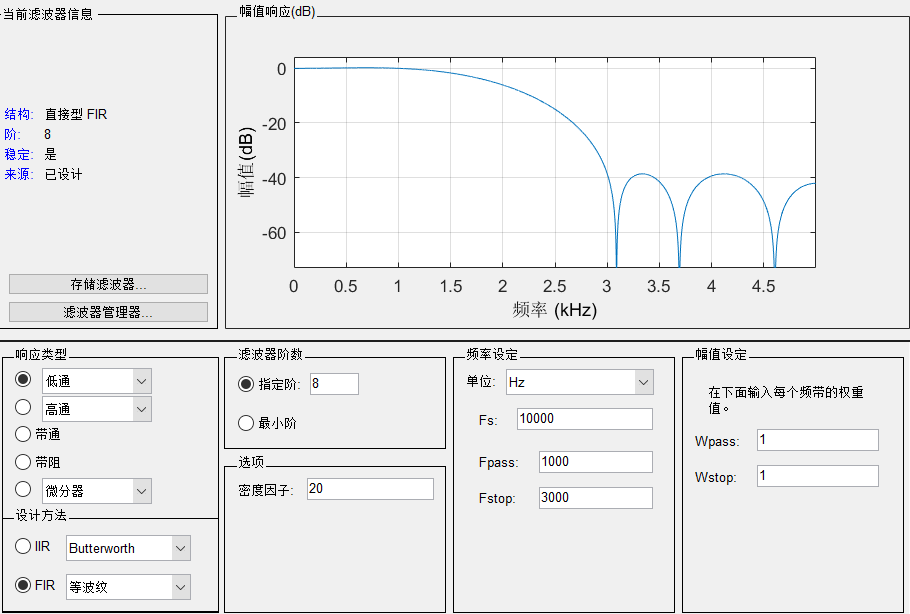
\includegraphics[width=1\textwidth]{part2_1.png}
    \caption{Filter Design Setting in Matlab filterDesigner Toolbox.}
\end{figure}
After setting these parameters and use the toolbox to design the filter, the coefficients can be exported to Matlab work-space. However, original generated coefficients are decimals, which are difficult to deal with in our system. It's necessary to convert these coefficients into integers. There's not only one conversion method, as long as to convert these decimals into a small range, this conversion method is feasible. Our conversion method is shown in the figure below:
\begin{figure}[H]
    \centering
    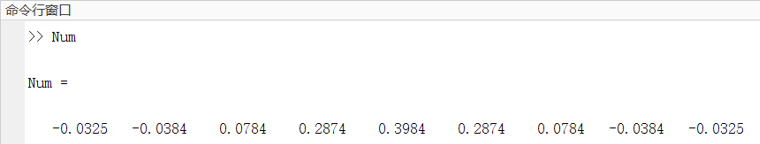
\includegraphics[width=1\textwidth]{part2_2.png}
    \caption{Original Coefficients from filterDesigner toolbox.}
\end{figure}
\begin{figure}[H]
    \centering
    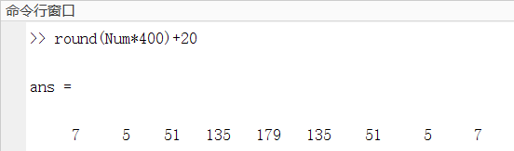
\includegraphics[width=1\textwidth]{part2_3.png}
    \caption{Converted Integer Coefficients.}
\end{figure}

\subsection{Filter Simulation in Matlab}
A simulation is also carried out in Matlab to obtain the expected results, which can be further used to compare to simulation result in Vivado. The digital sampling frequency is always keeping constant: $F_s = 10kHz$. The number of points of sampled discrete signal is N = 4096. To test the function of our filter, we mix 3 frequency components together to make it as the input of our system. The input signal consists of 3 mixed frequency: 1kHz, 3kHz, and 4kHz. We put our converted coefficients obtained from previous section into the simulation system, to verify function correctness of our design. As a low-pass filter, the theoretical result should be: signal with frequency 1kHz. The Matlab simulation result is shown in the figure below, which verifies that our designed coefficients can lead to correct results:
\begin{figure}[H]
    \centering
    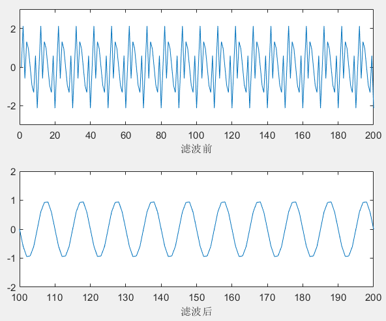
\includegraphics[width=1\textwidth]{part2_4.png}
    \caption{Simulation Results before and after Filtering.}
\end{figure}
Besides, in order to carry out the simulation in Vivado conveniently, we store the sampled discrete signal into a file, which will be read into a "memory" in Vivado simulation testbench. This procedure is done by Matlab script, which has been attached in the appendix section.

\section{Verilog Design and Simulation in Vivado -- Three implementations}
\subsection{Methodology 1: Direct Form Structure.}
The direct forrm structure is the normal structure in FIR design. We regard it as the basic one to implement.
\subsubsection{Architecture}
The Direct Form Structure take one input signal per clock cycle and save them into pipeline registers. The data in these registers will do multiplication with coefficient stored in multiplier, shown in diagram as h[i]. Then these the data result after multiplication will add together using an add as the filtered signal output.
\begin{figure}[H]
    \centering
    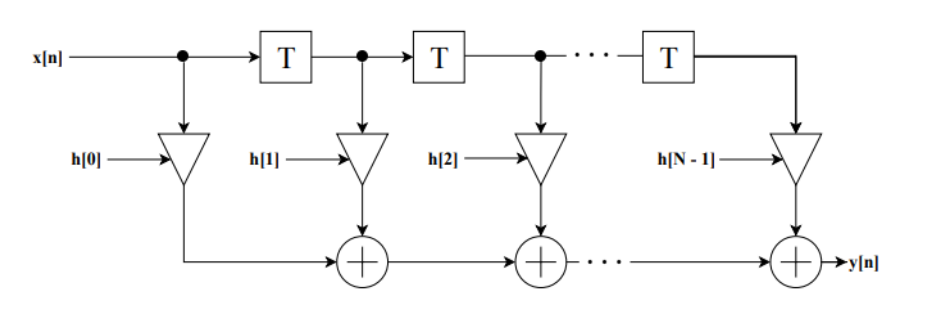
\includegraphics[width=1\textwidth]{siyuan/Direct structure.png}
    \caption{Diagram for Direct Form Structure.}
\end{figure}

\subsubsection{Schematic of Vivado Implementation Design}
The following figure is the schematic generated from Vivado.
\begin{figure}[H]
    \centering
    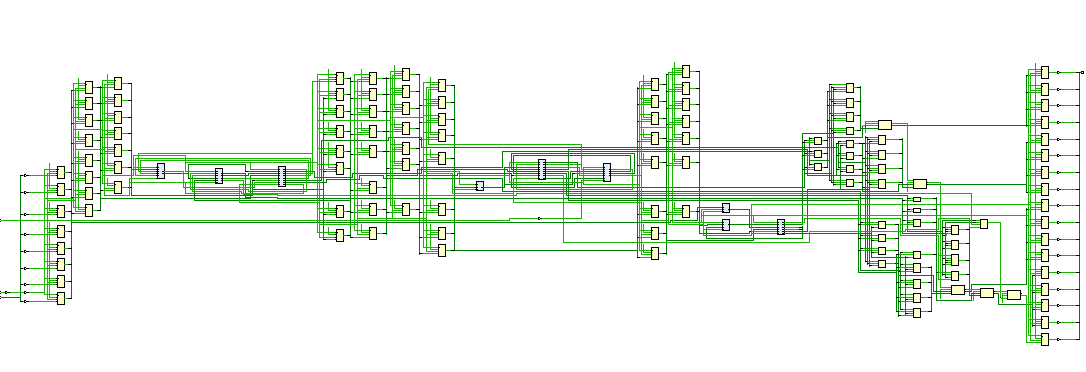
\includegraphics[width=1\textwidth]{siyuan/Direct schematic.png}
    \caption{Schematic for Direct Form Structure.}
\end{figure}

\subsubsection{Vivado Simulation}
The following screenshot is taken from simulation in Vivado running our designed test bench. The first wave that looks not so regular is our input. We generated it by mix three difference frequencies of sine waves. The second wave below is our output. It is the sine wave with 1k frequency. This simulation results is same as the simulation in Matlab, which means our low pass Direct Form FIR design is successful.
\begin{figure}[H]
    \centering
    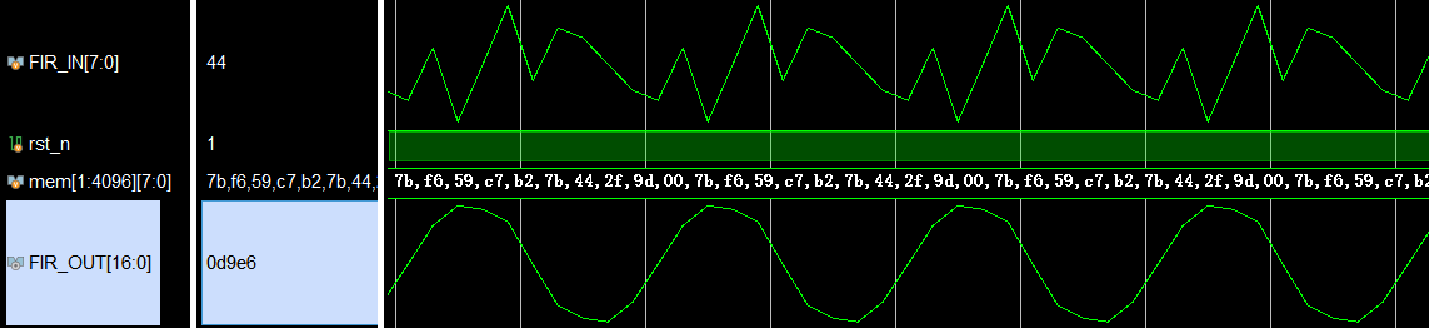
\includegraphics[width=1\textwidth]{siyuan/Direct simulation.png}
    \caption{Simulation result of Direct Form Structure.}
\end{figure}

\subsubsection{Implementation Design Report Checking: Power, Resource Utilization, and Timing}
In addition to analog simulation results, we also need to check other important properties of our design. They are power, resource utilization and timing.

This figure shows the power distribution of Direct Form Structure. Under default settings for power, the I/O consumes a large portion of power. 
\begin{figure}[H]
    \centering
    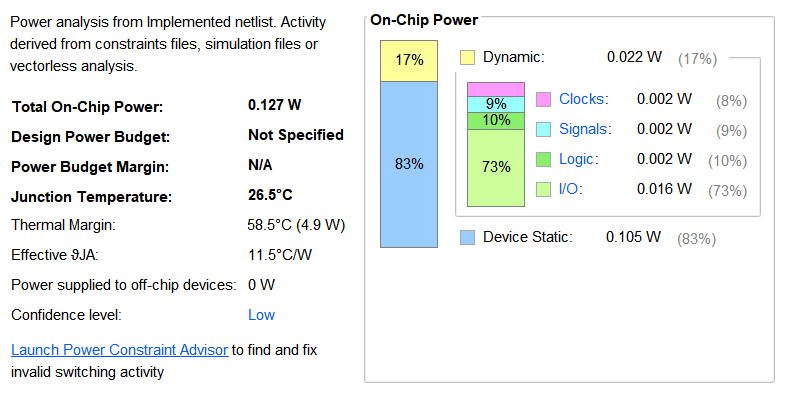
\includegraphics[width=1\textwidth]{siyuan/Direct power.png}
    \caption{Power summary for Direct Form Structure.}
\end{figure}

The summary of resource utilization report is:
\begin{figure}[H]
    \centering
    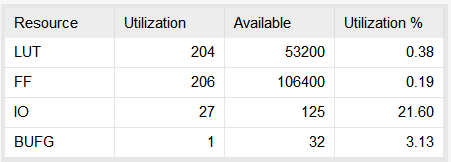
\includegraphics[width=0.8\textwidth]{siyuan/Direct usage.png}
    \caption{Resource Utilization Summary for Direct Form Structure.}
\end{figure}
Th timing report summary is shown below, where all timing constraints are met:
\begin{figure}[H]
    \centering
    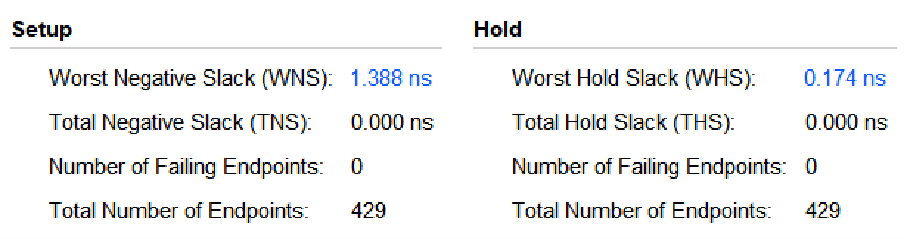
\includegraphics[width=1\textwidth]{siyuan/Direct timing.png}
    \caption{Timing Summary for Direct Form Structure}
\end{figure}
\subsection{Methodology 2: Symmetry Structure}

After generating coefficients from Matlab, we found that these coefficients are symmetric. After looking up signal processing books, these features were confirmed and we decided to take advantage of this principle. For example, if we want to build an 8-step FIR, we need 9 coefficients. We can use the following figure to represent this 9 values.
\begin{figure}[H]
    \centering
    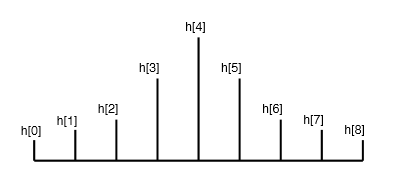
\includegraphics[width=1\textwidth]{siyuan/Sym coefficient.png}
    \caption{The Coefficient Feature.}
\end{figure}
Since there are only five different coefficient values, we can modify our design in the following structure.

\subsubsection{Architecture}
Taking advantage of the symmetric coefficients, we use the architecture shown below. In this Symmetry Structure design, we take one input signal per clock cycle and save them into pipeline registers. The data in these registers will do multiplication with coefficient stored in multiplier. Unlike the previous direct form one, the first pipeline register and the last pipeline register use one multiplier together. Therefore, in this structure, we can save 4 multipliers.
\begin{figure}[H]
    \centering
    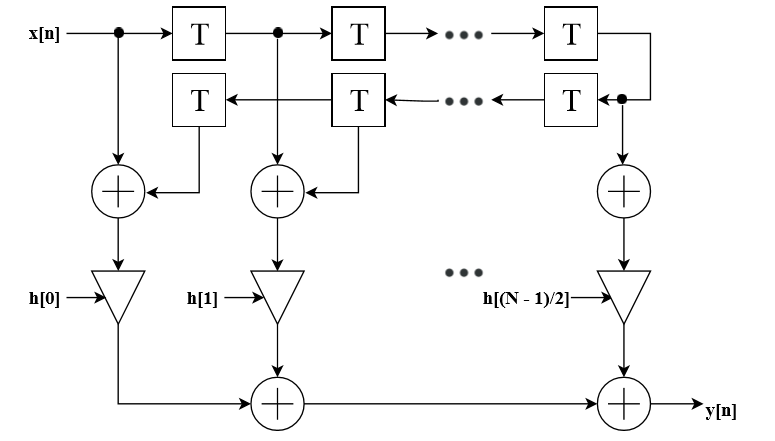
\includegraphics[width=1\textwidth]{siyuan/Sym structure.png}
    \caption{Diagram for Direct Form Structure.}
\end{figure}

\subsubsection{Schematic of Vivado Implementation Design}
The following figure is the schematic generated from Vivado.
\begin{figure}[H]
    \centering
    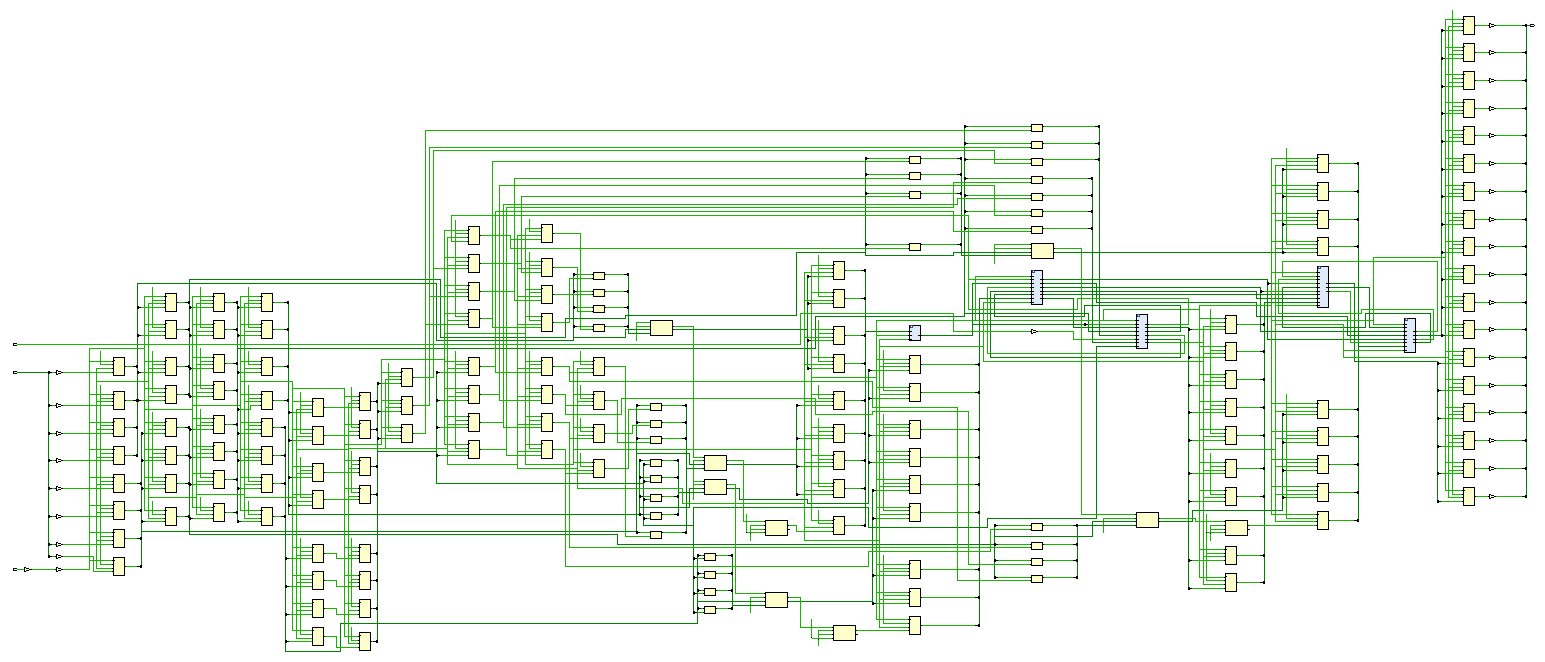
\includegraphics[width=1\textwidth]{siyuan/Sym schematic.png}
    \caption{Schematic for Symmetry Structure.}
\end{figure}

\subsubsection{Vivado Simulation}
The following screenshot is taken from simulation in Vivado running our designed test bench. The first wave that looks not so regular is our input. We generated it by mix three difference frequencies of sine waves. The second wave below is our output. It is the sine wave with 1k frequency. This simulation results is same as the simulation in Matlab, which means our low pass Direct Form FIR design is successful.Basically the simulation result of Symmetry Structure in Vivado test is the same as the Direct Form Structure.
\begin{figure}[H]
    \centering
    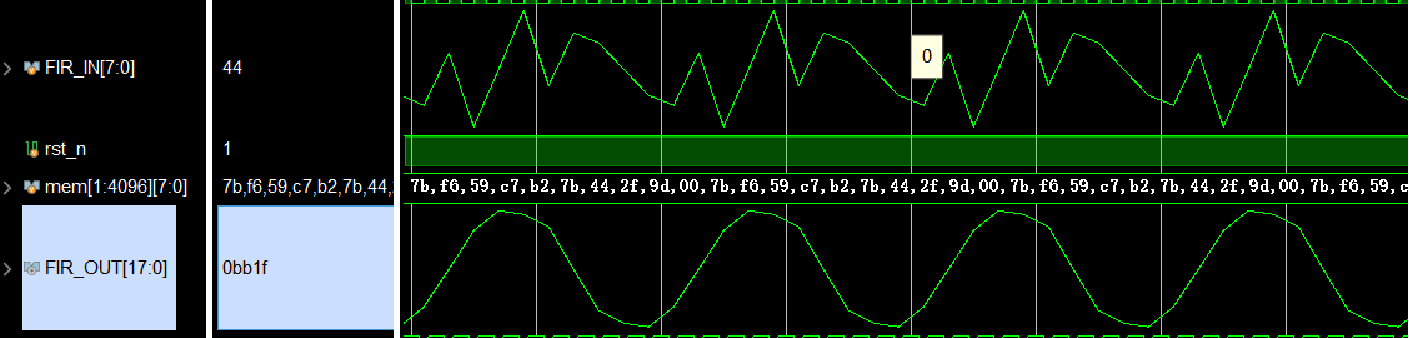
\includegraphics[width=1\textwidth]{siyuan/Sym simulation.png}
    \caption{Simulation result of Symmetry Structure.}
\end{figure}

\subsubsection{Implementation Design Report Checking: Power, Resource Utilization, and Timing}
Same as the previous section, we also need to check other important properties of our design. They are power, resource utilization and timing.

This figure shows the power distribution of Direct Form Structure. Under default settings for power, the I/O consumes a large portion of power. 
\begin{figure}[H]
    \centering
    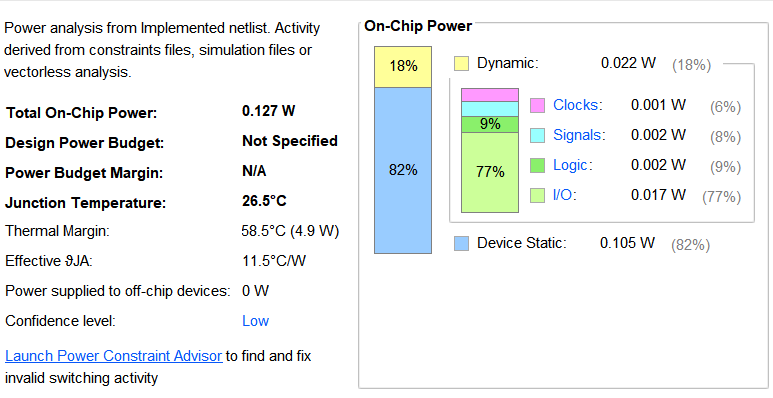
\includegraphics[width=1\textwidth]{siyuan/Sym power.png}
    \caption{Power summary for Symmetry Structure.}
\end{figure}

The summary of resource utilization report is:
\begin{figure}[H]
    \centering
    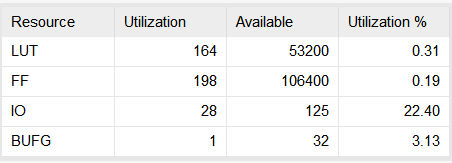
\includegraphics[width=0.8\textwidth]{siyuan/Sym usage.png}
    \caption{Resource Utilization Summary for Symmetry Structure}
\end{figure}
Th timing report summary is shown below, where all timing constraints are met:
\begin{figure}[H]
    \centering
    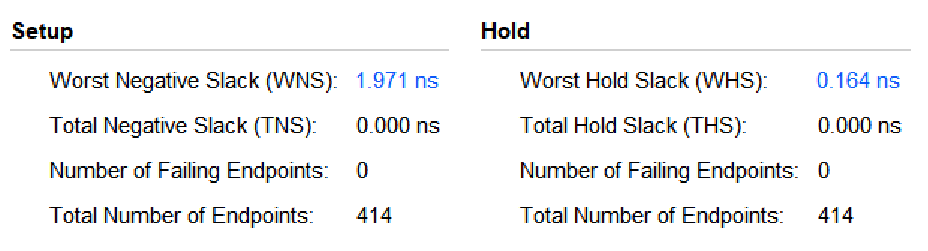
\includegraphics[width=1\textwidth]{siyuan/Sym timing.png}
    \caption{Timing Summary for Symmetry Structure.}
\end{figure}



\subsection{Methodology 3: Symmetry Structure with Xilinx Multiplier IPs}
\subsubsection{Architecture}
The multiplication in the FIR filter is to multiply the data with constant coefficients, which come from filter design specifications. We can make use this constant coefficient multiplication by replacing Vivado general synthesized x*y multiplier by Xilinx Multiplier IP, so that the logic can be simplified and the LUTs used by multipliers can be saved. The architecture is shown below, where each multiplier IP is written into corresponding coefficients. If the filter design changes, the IP should also be re-customized.
\begin{figure}[H]
    \centering
    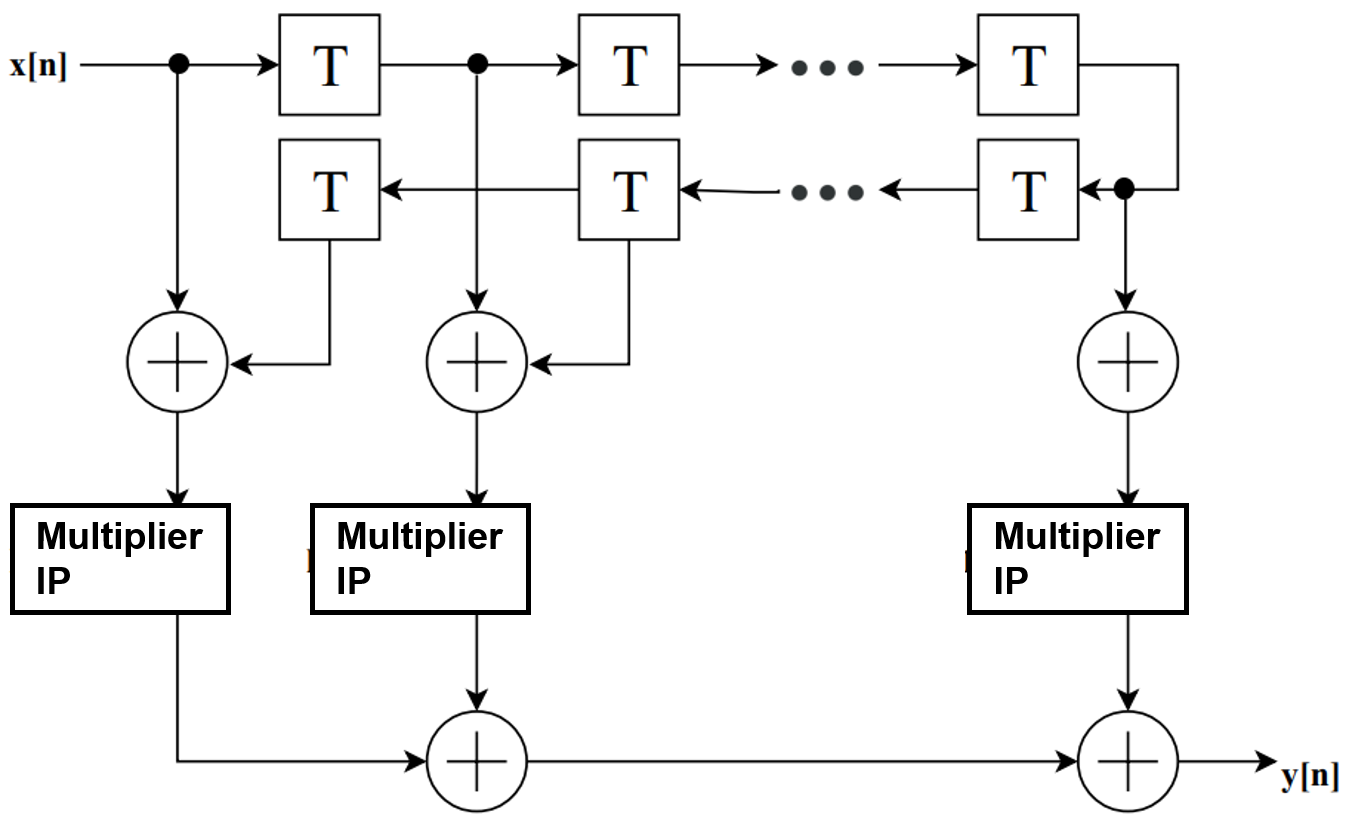
\includegraphics[width=1\textwidth]{part4_3_1.png}
    \caption{Architecture of Methodology 3.}
\end{figure}

\subsubsection{Schematic of Vivado Implementation Design}
The schematic of Vivado implementation design is:
\begin{figure}[H]
    \centering
    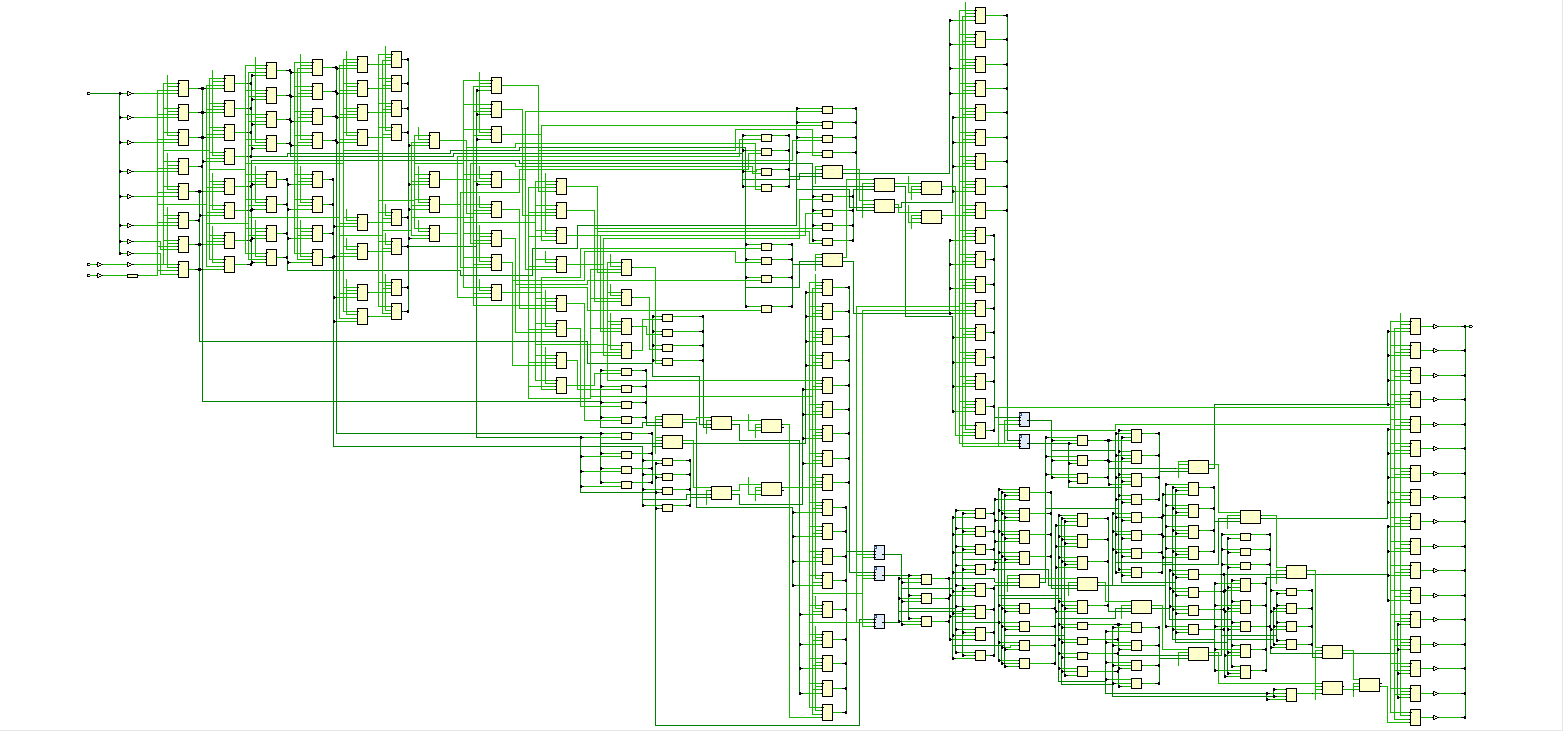
\includegraphics[width=1\textwidth]{part4_3_2.png}
    \caption{Implementation Design of Methodology 3.}
\end{figure}
\subsubsection{Vivado Simulation}
Similar to previous implementations, simulations are carried out to verify its function correctness. The simulation waveform is shown below, where the filter works properly:
\begin{figure}[H]
    \centering
    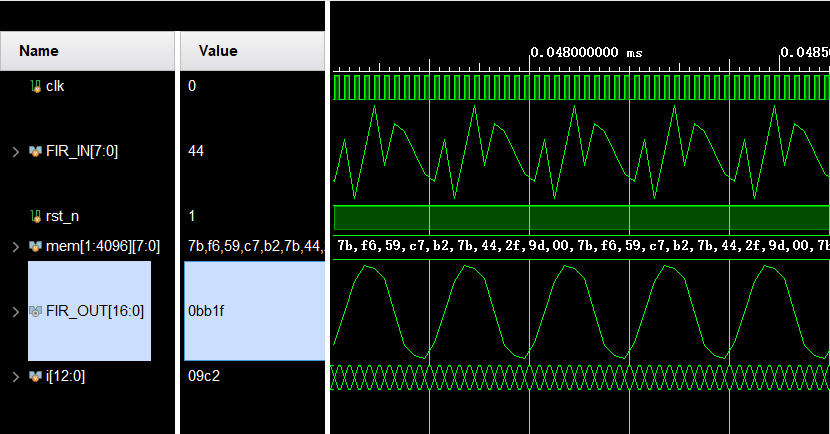
\includegraphics[width=1\textwidth]{part4_3_3.png}
    \caption{Simulation Waveform of Methodology 3.}
\end{figure}
\subsubsection{Implementation Design Report Checking: Power, Resource Utilization, and Timing}
Under default settings for power, the power report summary is shown below. The I/O consumes a large portion of power in this implemented design, by carefully inspecting the power report of I/O, we find that the 16-bit output of our FIR filter consumes a lot of power. In fact, each port consumes a small amount of power of less than 0.001w, but 16 ports together make the portion of total power large. 
\begin{figure}[H]
    \centering
    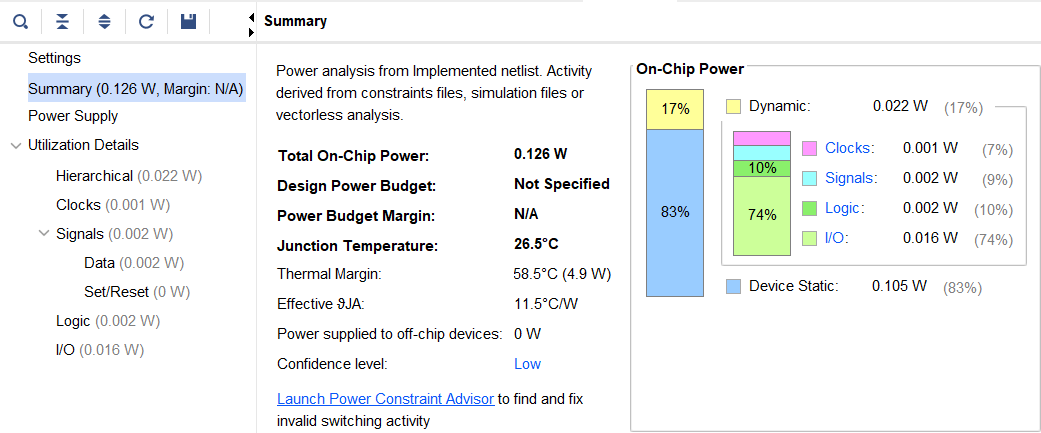
\includegraphics[width=1\textwidth]{part4_3_4_1.png}
    \caption{Power Report Summary of Methodology 3.}
\end{figure}

The hierarchy and summary of resource utilization report is:
\begin{figure}[H]
    \centering
    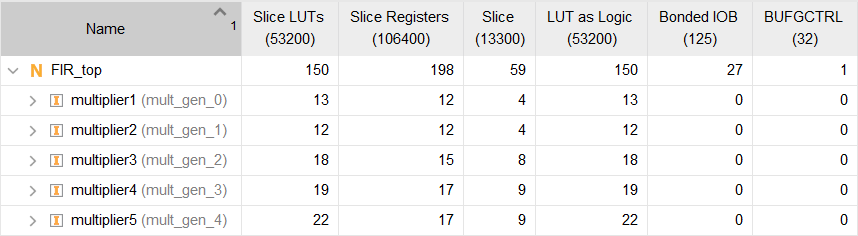
\includegraphics[width=1\textwidth]{part4_3_4_2_1.png}
    \caption{Utilization Report of Hierarchy.}
\end{figure}
\begin{figure}[H]
    \centering
    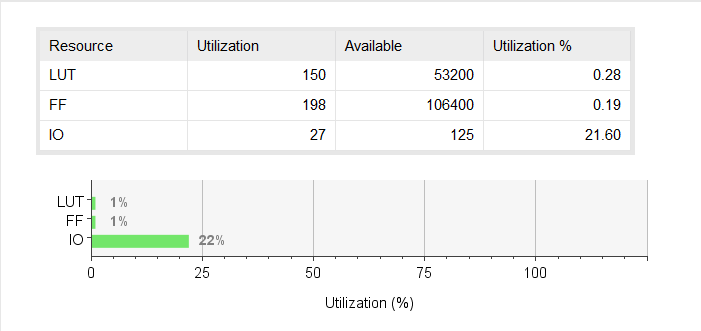
\includegraphics[width=1\textwidth]{part4_3_4_2_2.png}
    \caption{Utilization Report Summary.}
\end{figure}

The timing report summary is shown below, where all timing constraints are met:
\begin{figure}[H]
    \centering
    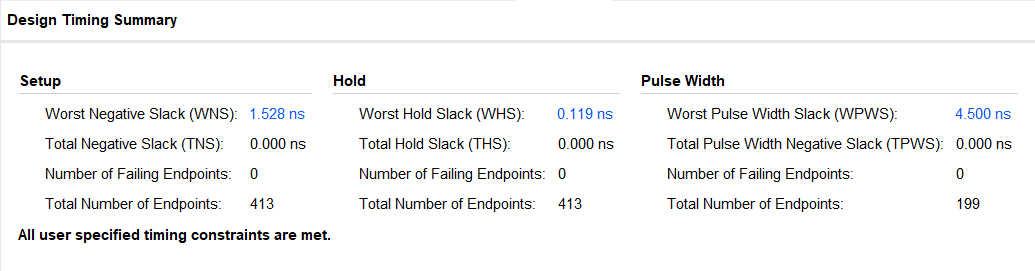
\includegraphics[width=1\textwidth]{part4_3_4_3.png}
    \caption{Timing Summary Report.}
\end{figure}

\subsection{Comparison of 3 Design Implementations}
So far we have developed three methodologies for FIR. In this section, we will have a comparison among these three structures to see how we improved how design steps by steps.
\subsubsection{Timing Comparison}
The following table shows the timing comparison among three structures. There are not critical timing issues. That is the total negative slack and total hold slack for these three methodologies are 0. As for the worst negative slack(WNS) and worst hold slack(WHS), there are slightly differences. The greater the WNS and WHS, the more difficult this structure meets timing issues.
\begin{table}[]
\centering
\begin{tabular}{ccccl}
\cline{1-4}
\multicolumn{1}{|c|}{Timing(ns)}           & \multicolumn{1}{c|}{Direct} & \multicolumn{1}{c|}{Symmetry} & \multicolumn{1}{c|}{Symmetry with Multiplier IP} &  \\ \cline{1-4}
\multicolumn{1}{|c|}{Worst Negative Slack} & \multicolumn{1}{c|}{1.388}  & \multicolumn{1}{c|}{1.971}    & \multicolumn{1}{c|}{1.528}                       &  \\ \cline{1-4}
\multicolumn{1}{|c|}{Worst Hold Slack}     & \multicolumn{1}{c|}{0.174}  & \multicolumn{1}{c|}{0.164}    & \multicolumn{1}{c|}{0.119}                       &  \\ \cline{1-4}
\multicolumn{1}{|c|}{Total Negative Slack} & \multicolumn{1}{c|}{0} & \multicolumn{1}{c|}{0} & \multicolumn{1}{c|}{0} &  \\ \cline{1-4}
\multicolumn{1}{|c|}{Total Hold Slack}     & \multicolumn{1}{c|}{0} & \multicolumn{1}{c|}{0} & \multicolumn{1}{c|}{0} &  \\ \cline{1-4}
                                           &                        &                        &                        &  \\
                                           &                        &                        &                        & 
\end{tabular}
\caption{Timing Comparison of Three Methodologies}
\end{table}

\subsubsection{Source Utilization Comparison}
The following table shows the source utilization of different methodologies. The Direct Form Structure uses most. The Symmetry Structure uses less because the number of multipliers is saved by half. The Symmetry Structure with Multiplier IP uses the least. The reason is mentioned in 4.3.1. By comparison, it turns out that our improvement in structures works.
\begin{table}[]
\centering
\begin{tabular}{ccccl}
\cline{1-4}
\multicolumn{1}{|c|}{Source Utilization} & \multicolumn{1}{c|}{Direct} & \multicolumn{1}{c|}{Symmetry} & \multicolumn{1}{c|}{Symmetry with Multiplier IP} &  \\ \cline{1-4}
\multicolumn{1}{|c|}{LUT} & \multicolumn{1}{c|}{204} & \multicolumn{1}{c|}{164} & \multicolumn{1}{c|}{150} &  \\ \cline{1-4}
\multicolumn{1}{|c|}{FF}  & \multicolumn{1}{c|}{206} & \multicolumn{1}{c|}{198} & \multicolumn{1}{c|}{198} &  \\ \cline{1-4}
                          &                          &                          &                          &  \\
                          &                          &                          &                          &  \\
                          &                          &                          &                          &  \\
                          &                          &                          &                          & 
\end{tabular}
\caption{Source Utilization Comparison of Three Methodologies}
\end{table}

\subsubsection{Power Comparison}
From power report above, we can observe that all methods seem to have the same power consumption, where I/Os consume a large portion of power. The main reason is that we use many ports for 8-bit input sequence and 16-bit output sequence. Also since our design is a bit small, the logic and timing power is very small, which makes I/Os become a large part of power consumption.

\section{ZYNQ Implementation on Arty Z7 Board}
In this part, we designed an IP package and a simple application that transfer computation to Arty Z7 board.
\subsection{IP Block Design}
\begin{figure}[H]
    \centering
    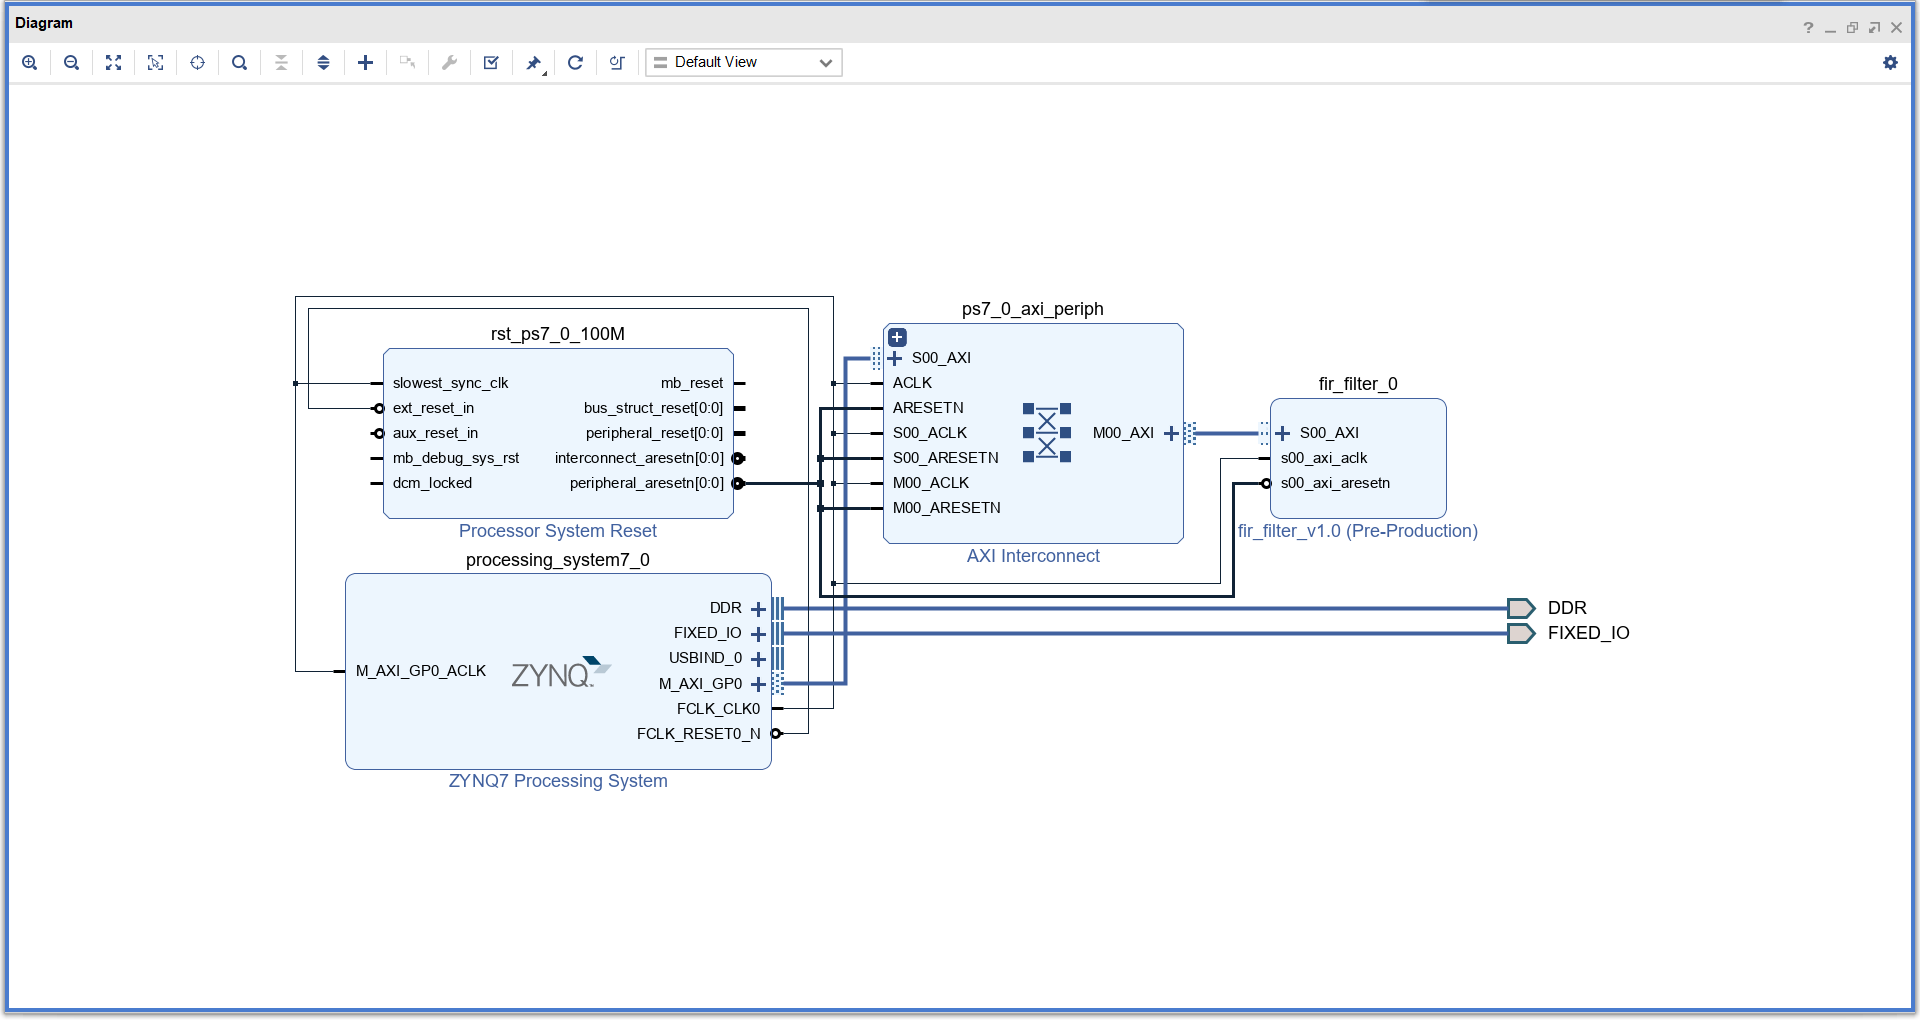
\includegraphics[width=1\textwidth]{diagram.png}
    \caption{IP Package Design.}
\end{figure}
We first create a new Xilinx Vivado project and create and package a new IP.
\begin{table}[H]
    \centering
    \begin{tabular}{|c|c|}
        \hline
        Name&S00\_AXI\\
        \hline
        Interface Type&Lite\\
        \hline
        Interface Mode&Slave\\
        \hline
        Data Width (Bits)&32\\
        \hline
        Memory Size (Bytes)&64\\
        \hline
        Number of Registers&11\\
        \hline
    \end{tabular}
    \caption{AXI Interfaces of IP \protect\footnotemark}
\end{table}
\footnotetext{Data Width is standard 32 bits of AXI bus not changeable, although we only need 17 bits.}
Editing IP, we add design sources and modify the code of instance. Then. changes are merged in file groups and IP is re-packaged. After the IP block is ready, we create a block design. In the block design, first add ZYNQ 7 Processing System (\texttt{processing\_system7\_0}) and connect \texttt{DDR}, \texttt{FIXED\_IO}, \texttt{FCLK\_CLK0}, and \texttt{M\_AXI\_GP0\_ACLK}. Then from the Verilog design of FIR filter, we derive an IP block \texttt{fir\_filter\_v1.0 (Pre-Production)} (\texttt{fir\_filter\_0}), and connect its \texttt{s00\_axi\_aclk} to \texttt{FCLK\_CLK0} and \texttt{M\_AXI\_GP0\_ACLK} of \texttt{processing\_system7\_0} and \texttt{slowest\_sync\_clk} of Processor System Reset (\texttt{rst\_ps7\_0\_100M}) to synchronize the clocks. Then, we connect \texttt{s00\_axi\_aresetn} of \texttt{fir\_filter\_0} to \texttt{ARESETN} of AXI Interconnect (\texttt{ps7\_0\_axi\_periph}) and \texttt{peripheral\_aresetn[0:0]} of \texttt{rst\_ps7\_0\_100M} to enable RESET. Finally, we connect \texttt{S00\_AXI} of \texttt{fir\_filter\_0} to \texttt{M00\_AXI} of \texttt{ps7\_0\_axi\_periph} to transfer data via AXI bus.
\subsection{Vivado Hardware}
After block design is ready, we create an HDL wrapper for the block design, let Vivado to manage wrapper and auto-update, run synthesis, run implementation, and generate bitstream.
\begin{figure}[H]
    \centering
    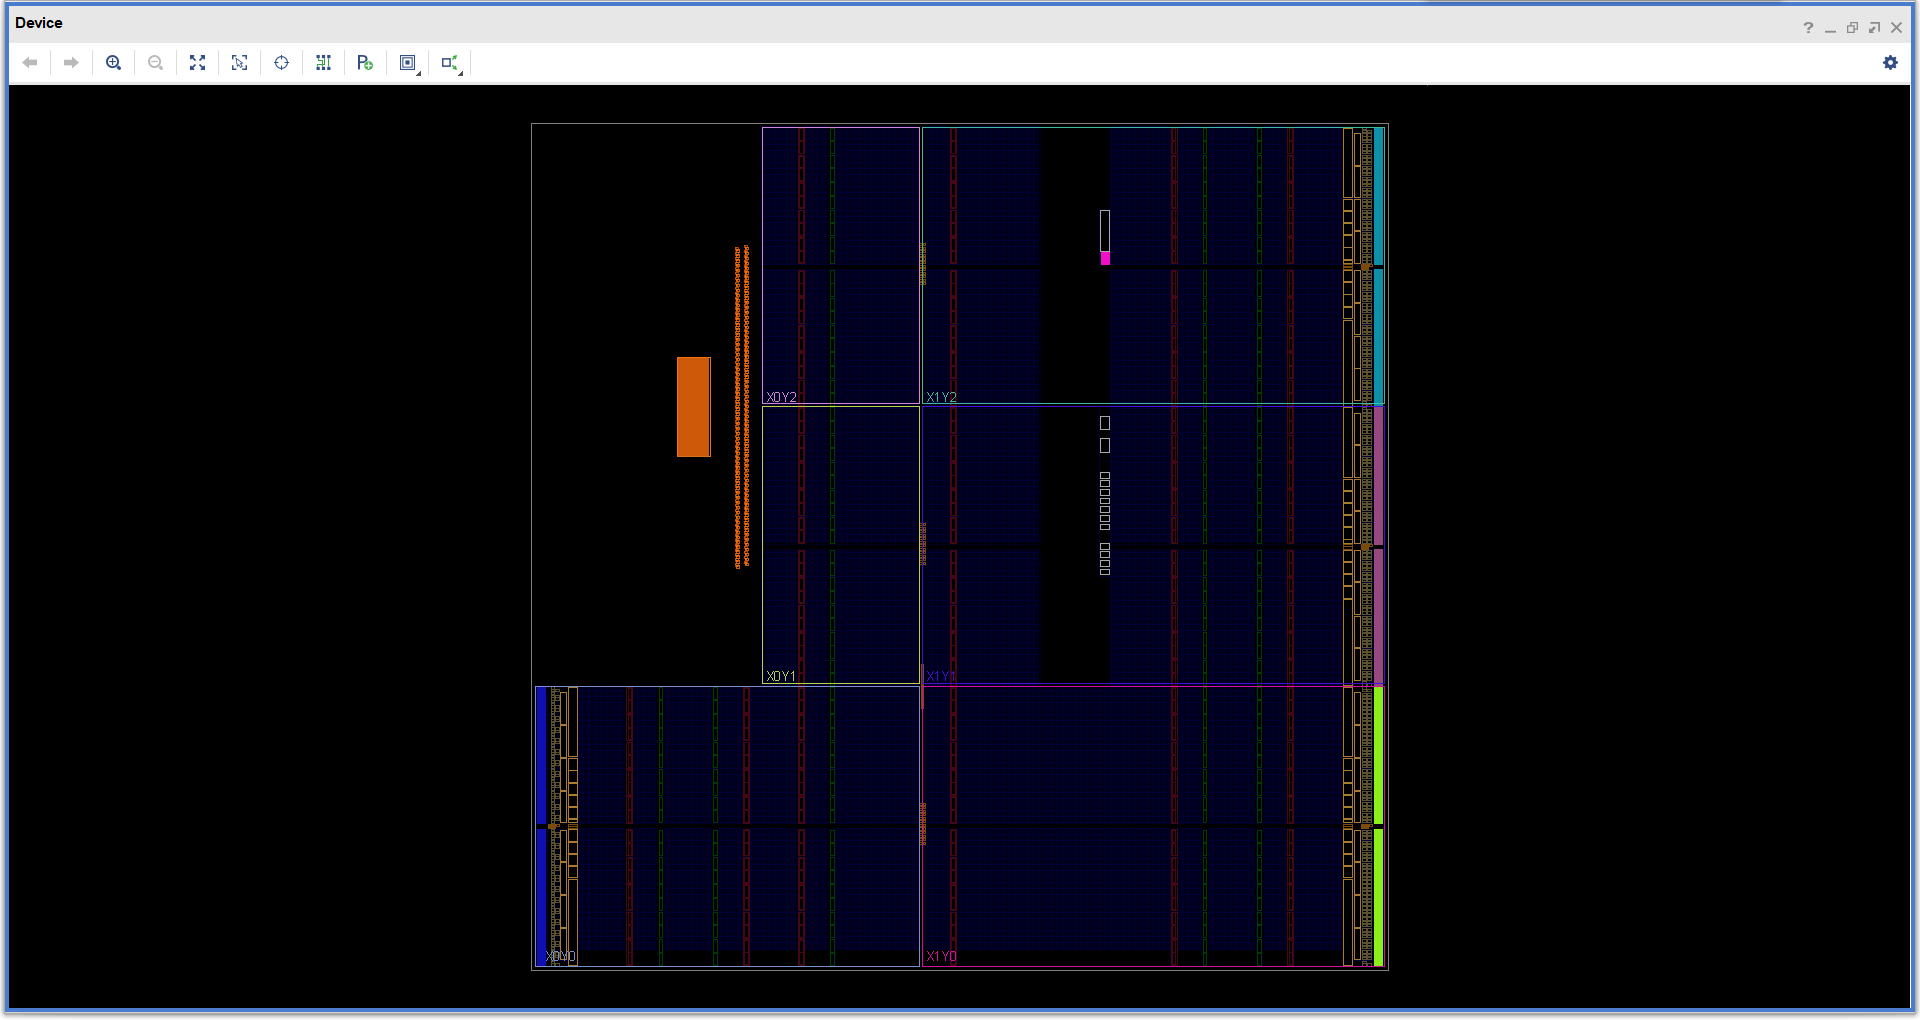
\includegraphics[width=1\textwidth]{syn.png}
    \caption{Synthesis design.}
\end{figure}
\begin{figure}[H]
    \centering
    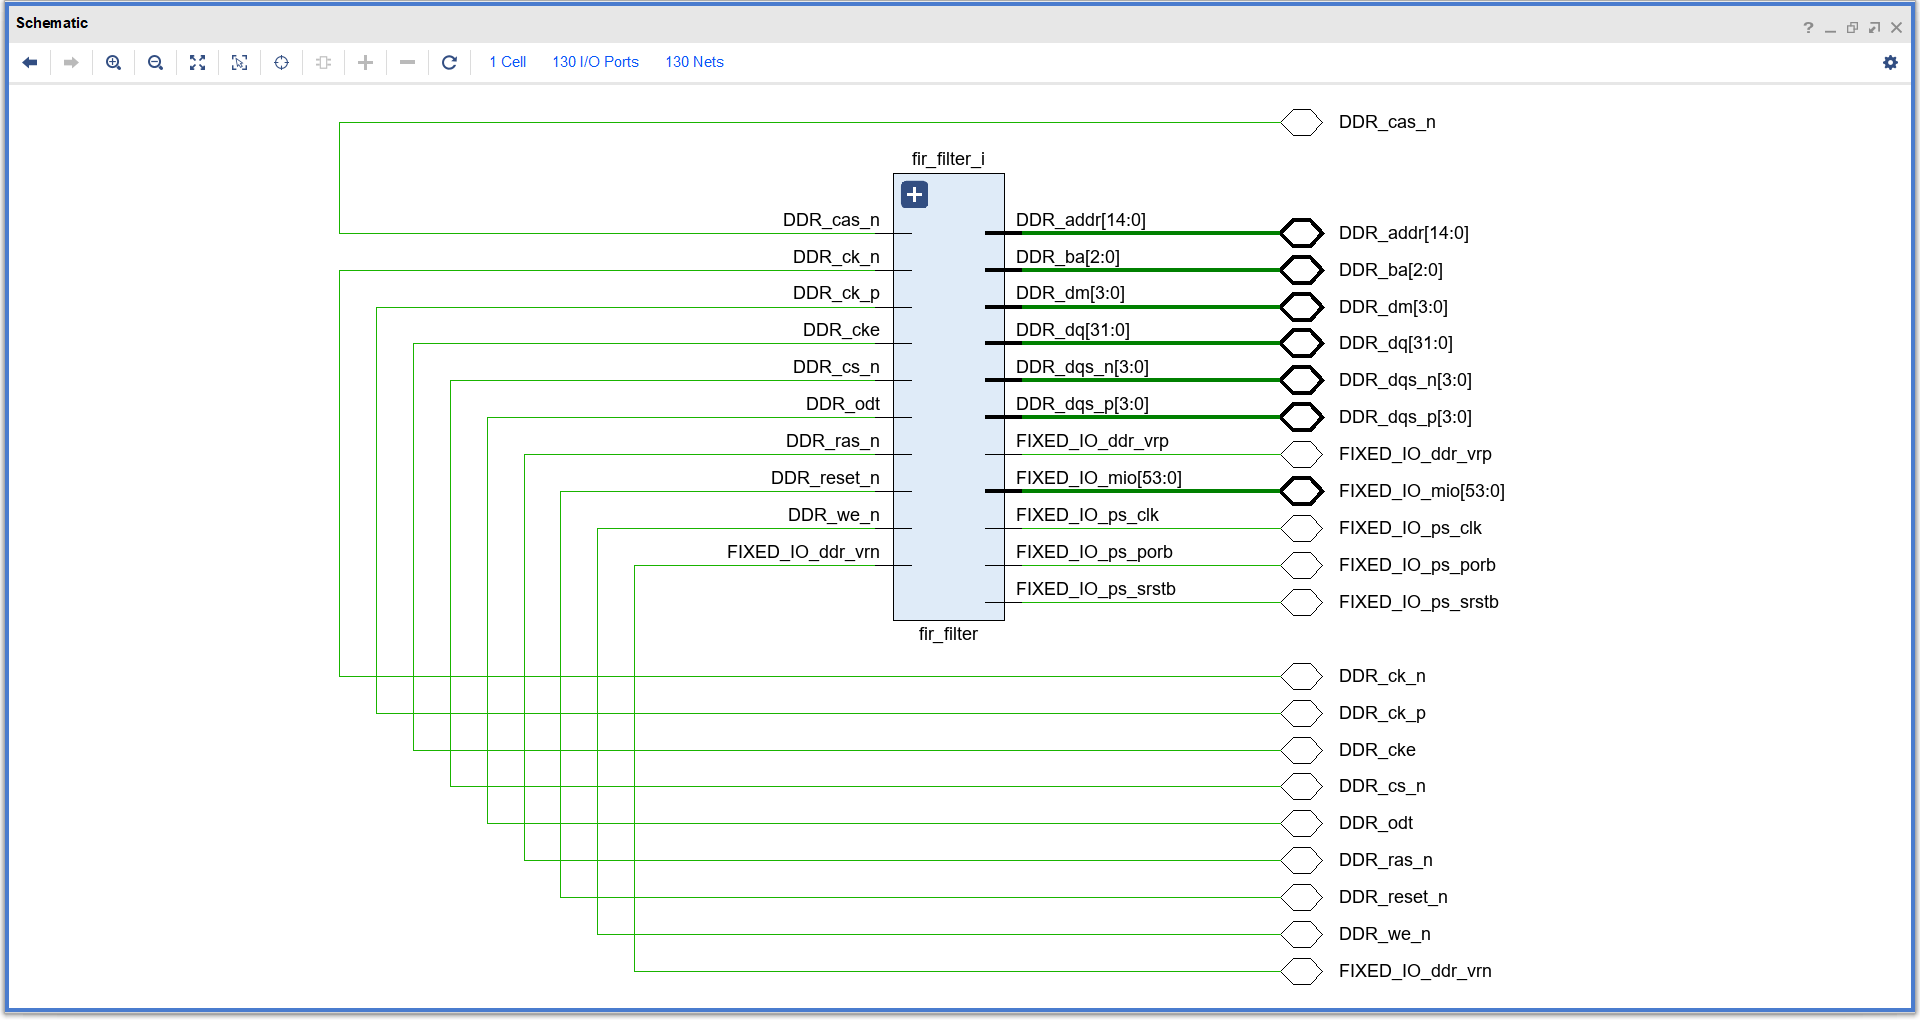
\includegraphics[width=1\textwidth]{sch.png}
    \caption{Schematic diagram.}
\end{figure}
\begin{figure}[H]
    \centering
    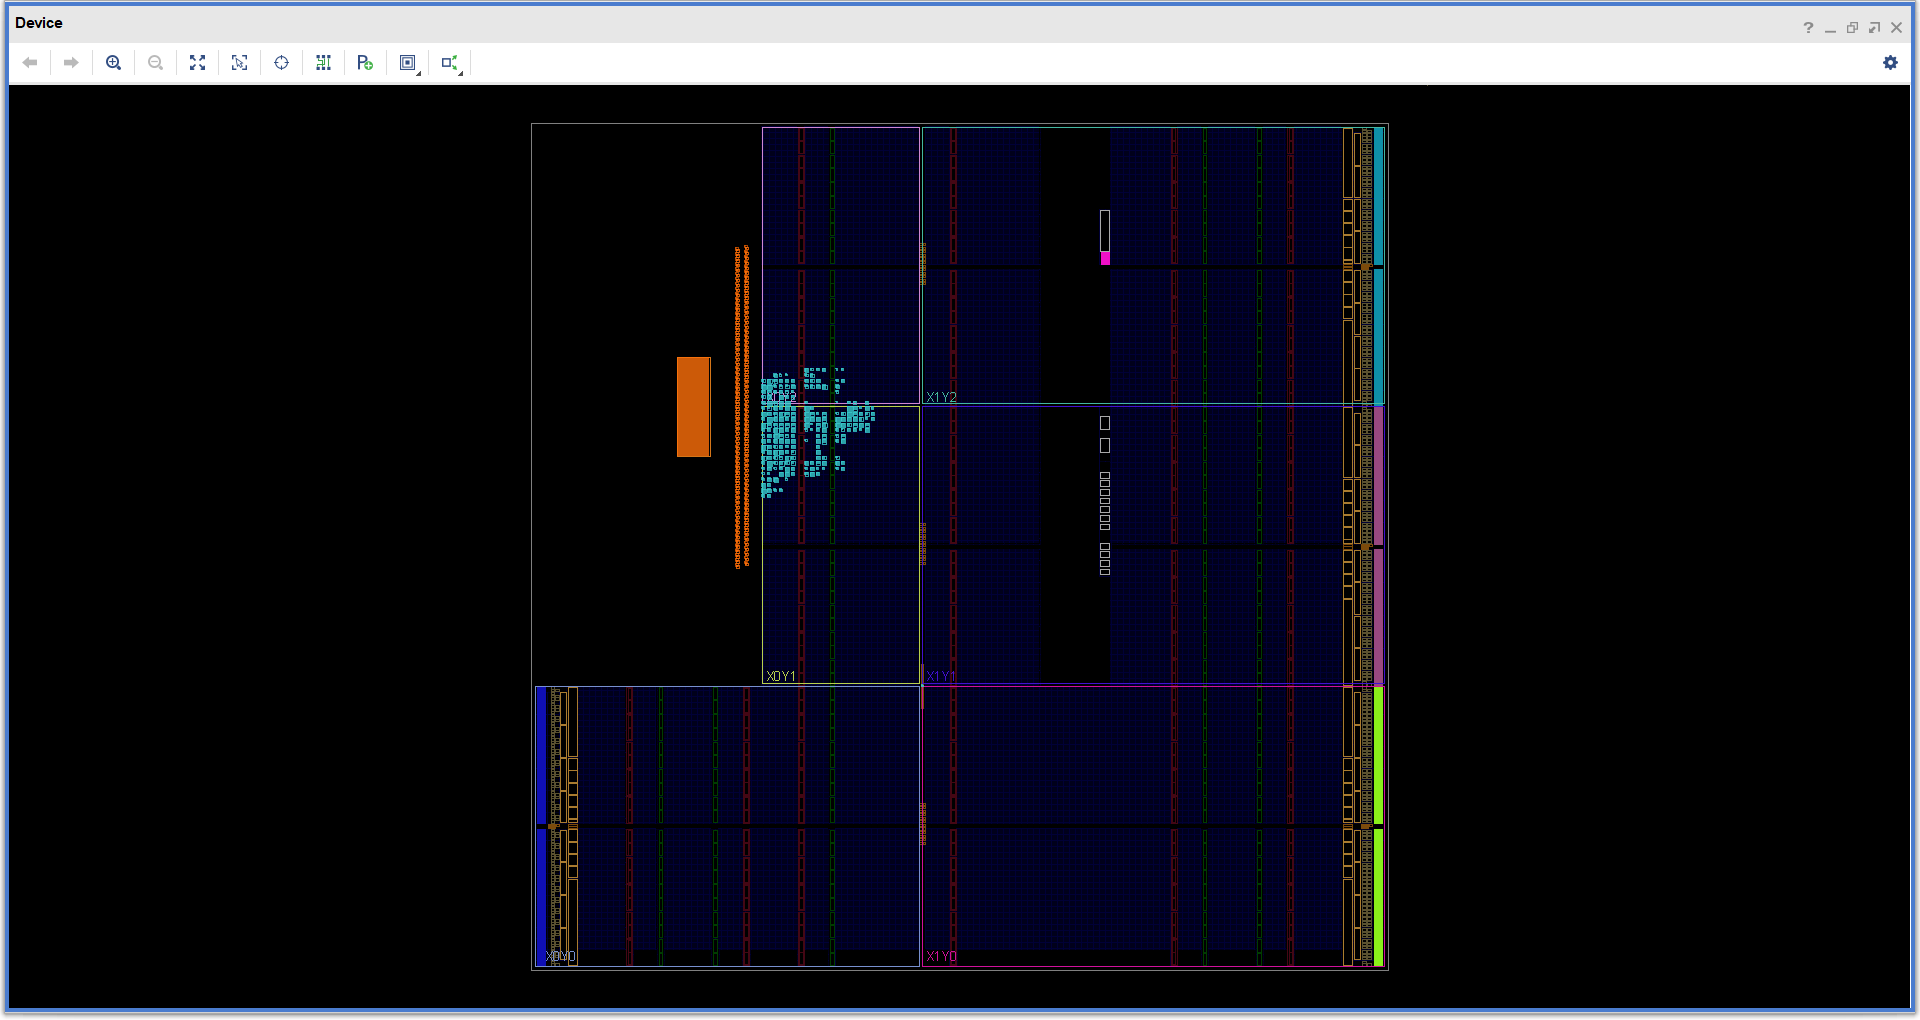
\includegraphics[width=1\textwidth]{impl.png}
    \caption{Implementation design.}
\end{figure}
After bitstream is ready, we export the hardware for Vitis use.
\subsection{Vitis Application}
In Vitis, we create an application project with OS platform is standalone and processor is \texttt{ps7\_cortexa9\_0} and make use of the previously exported XSA wrapper file. Then, we pick the first hexadecimal number from the previously generated memory and examine the input and output of the FIR filter IP. Still we have to resolve the bug of Xilinx Vitis 2021.1.1. This bug can cause different errors.
\begin{itemize}
    \item Modify \texttt{fir\_filter\_hdl\_wrapper/zynq\_fsbl/zynq\_fsbl\_bsp/ps7\_cortexa9\_0/ libsrc/fir\_filter\_v1\_0/src/Makefile} and \texttt{fir\_filter\_hdl\_wrapper/
    ps7\_cortexa9\_0/standalone\_ps7\_cortexa9\_0/bsp/ps7\_cortexa9\_0/libsrc/
    fir\_filter\_v1\_0\_v1\_0/src/Makefile} (see Appendix).
    \item Create a new directory \texttt{qemu} under \texttt{fir\_filter\_hdl\_wrapper/export/fir\_filter\_hdl\_wrapper/
    sw/fir\_filter\_hdl\_wrapper}.
    \item Create an empty file \texttt{qemu\_args.txt} under the newly created directory.
\end{itemize}
After building finished, we have to set up FPGA.
\begin{itemize}
    \item Connect USB between FPGA and the computer.
    \item JP4 jumper is set as JTAG mode.
    \item JP5 jumper is set as USB mode.
    \item In Device Manager of Windows, go to ports, change the USB Serial Port Properties of COM4 as
\begin{table}[H]
    \centering
    \begin{tabular}{|c|c|}
        \hline
        Bits per second&115200\\
        \hline
        Data bits&8\\
        \hline
        Parity&None\\
        \hline
        Stop bits&1\\
        \hline
        Flow control&None\\
        \hline
    \end{tabular}
    \caption{USB Serial Port Properties of COM4.}
\end{table}
\end{itemize}
\begin{figure}[H]
    \centering
    \includegraphics[width=0.8\textwidth]{fpga.jpg}
    \caption{FPGA set-up.}
\end{figure}
we connect FPGA to the computer through USB, run as launching on hardware (GDB), open and set Vitis Serial Terminal to connect to a serial port with the following settings:
\begin{table}[H]
    \centering
    \begin{tabular}{|c|c|}
        \hline
        Port&COM4\\
        \hline
        Baud Rate&115200\\
        \hline
        Data Bits&8\\
        \hline
        Stop Bits&1\\
        \hline
        Parity&None\\
        \hline
        Flow Control&None\\
        \hline
    \end{tabular}
    \caption{Basic and advance settings of Vitis Serial Terminal to connect to serial port.}
\end{table}
Observe in Vitis Serial Terminal.
\begin{figure}[H]
    \centering
    \includegraphics[width=0.6\textwidth]{vitis_app_term.png}
    \caption{Screenshot of the Vitis Serial Terminal.}
\end{figure}
Here we can observe that the input is 8 bits and the output is 17 bits, and the output is the correct output.
\section{Discussion and Conclusion}

As a brief summary, this project goes through the whole design flow of an FIR filter from digital signal sampling and filter coefficients design in Matlab down to hardware implementation on FPGA. We implement the A/D conversion in Matlab and store the converted file with digital signal in a file. This file will be used in Vivado simulation testbench to read in the digital signal. The back-end D/A conversion can be automatically executed in Vivado during simulation. In reality, a 8-bit DAC is expected to convert the filtered signal as analog. Three implementations are implemented on FPGA and simulation verifies all three versions work correctly. Comparisons are carried out among 3 methods, by using symmetry structure, the multiplier usage can be reduced by half, which can significantly save the resource consumption. Since the constant multiplication in FIR filter, using Xilinx Multiplier IP can also help to reduce the resource utilization. ZYNQ implementation also shows that this design can be packaged in to an IP and used as an accelerator of ZYNQ processing system. 

There are also many potential improvements of FIR filter implementation on FPGA. Due to time limitation, we are not able to do them.The number of tap and bit width can be increased, so that the filter is closer to real applications. A large tap FIR filter with complex structure can greatly reveal the advantage of improvements in our method 2 and 3. Since our design is still, to some extent, in small scale, these improvements are not so apparent. For a large filter, we can also make use of DSP blocks on FPGA to save the computation resource consumption. Another improvement could be approximate computing. Since our design is not large, we finally decide not to implement this since it will largely reduce the performance with very little improvement in timing. But it will benefits a lot for a large filter. We also studied many approximate algorithm during literature research, such as 4-2 compressor in multiplication. 
\section{References}
\noindent [1] \url{https://conferences.computer.org/ictapub/pdfs/ITCA2020-6EIiKprXTS23UiQ2usLpR0/114100a079/114100a079.pdf}

\noindent [2] \url{https://liu.diva-portal.org/smash/get/diva2:1256720/FULLTEXT01.pdf}

\noindent [3] Lars Wanhammar and Håkan Johansson. Digital filters using Matlab. Department of
Electrical Engineering, Linköping University, 2011.
\section{Appendix}
\subsection{MATLAB Code for Generating Memory for Simulation}
\inputminted[frame=single,bgcolor=bg,breaklines,breakanywhere,linenos]{matlab}{generate_mem.m}
\subsection{MATLAB Code for Simluation}
\inputminted[frame=single,bgcolor=bg,breaklines,breakanywhere,linenos]{matlab}{simulation.m}
\subsection{Verilog Code for FIR Filter}
\inputminted[frame=single,bgcolor=bg,breaklines,breakanywhere,linenos]{verilog}{FIR_top.v}
\subsection{Verilog Code for Multiplier}
\inputminted[frame=single,bgcolor=bg,breaklines,breakanywhere,linenos]{verilog}{multiplier.v}
\subsection{Part of Verilog Code of FIR Filter AXI Instance}
\begin{minted}[frame=single,bgcolor=bg,breaklines,breakanywhere,linenos]{verilog}
`timescale 1 ns / 1 ps

	module fir_filter_v1_0_S00_AXI(
	    // ...
	)
	(
	    // ...
	)
	// Implement memory mapped register select and read logic generation
	// Slave register read enable is asserted when valid address is available
	// and the slave is ready to accept the read address.
	assign slv_reg_rden = axi_arready & S_AXI_ARVALID & ~axi_rvalid;
	always @(*)
	begin
	      // Address decoding for reading registers
	      case ( axi_araddr[ADDR_LSB+OPT_MEM_ADDR_BITS:ADDR_LSB] )
	        2'h0   : reg_data_out <= slv_reg0;
	        2'h1   : reg_data_out <= FIR_top_out;
	        2'h2   : reg_data_out <= slv_reg2;
	        2'h3   : reg_data_out <= slv_reg3;
	        default : reg_data_out <= 0;
	      endcase
	end
	// ...
	// Add user logic here
    wire [17:0] FIR_top_out;
    FIR_top FIR_top_instance_01(
        .clk(S_AXI_ACLK),
        .rst_n(S_AXI_ARESETN),
        .FIR_IN(slv_reg0[7:0]),
        .FIR_OUT(FIR_top_out)
    );
	// User logic ends
	
	endmodule
\end{minted}
\subsection{Constraints of FIR Filter}
\inputminted[frame=single,bgcolor=bg,breaklines,breakanywhere,linenos]{text}{constraints.xdc}
\subsection{Verilog Code for FIR Filter Simulation}
\inputminted[frame=single,bgcolor=bg,breaklines,breakanywhere,linenos]{verilog}{FIR_test.v}
\subsection{C Code of Xilinx Vitis Application}
\inputminted[frame=single,bgcolor=bg,breaklines,breakanywhere,linenos]{c}{helloworld.c}
\subsection{Modified Makefile of FIR Filter HDL Wrapper}
\inputminted[frame=single,bgcolor=bg,breaklines,breakanywhere,linenos]{makefile}{Makefile}
\subsection{XILINX Core Generator(tm) Disributed Arithmetic FIR Filter Coefficient (.COE)}
\inputminted[frame=single,bgcolor=bg,breaklines,breakanywhere,linenos]{text}{FIR.coe}
\end{document}
